\documentclass{beamer}
\mode<presentation>
\usepackage{amsmath}
\usepackage{amssymb}
%\usepackage{advdate}
\usepackage{adjustbox}
\usepackage{subcaption}
\usepackage{enumitem}
\usepackage{multicol}
\usepackage{mathtools}
\usepackage{listings}
\usepackage{url}
\def\UrlBreaks{\do\/\do-}
\usetheme{Boadilla}
\usecolortheme{lily}
\setbeamertemplate{footline}
{
  \leavevmode%
  \hbox{%
  \begin{beamercolorbox}[wd=\paperwidth,ht=2.25ex,dp=1ex,right]{author in head/foot}%
    \insertframenumber{} / \inserttotalframenumber\hspace*{2ex} 
  \end{beamercolorbox}}%
  \vskip0pt%
}
\setbeamertemplate{navigation symbols}{}

\providecommand{\nCr}[2]{\,^{#1}C_{#2}} % nCr
\providecommand{\nPr}[2]{\,^{#1}P_{#2}} % nPr
\providecommand{\mbf}{\mathbf}
\providecommand{\pr}[1]{\ensuremath{\Pr\left(#1\right)}}
\providecommand{\qfunc}[1]{\ensuremath{Q\left(#1\right)}}
\providecommand{\sbrak}[1]{\ensuremath{{}\left[#1\right]}}
\providecommand{\lsbrak}[1]{\ensuremath{{}\left[#1\right.}}
\providecommand{\rsbrak}[1]{\ensuremath{{}\left.#1\right]}}
\providecommand{\brak}[1]{\ensuremath{\left(#1\right)}}
\providecommand{\lbrak}[1]{\ensuremath{\left(#1\right.}}
\providecommand{\rbrak}[1]{\ensuremath{\left.#1\right)}}
\providecommand{\cbrak}[1]{\ensuremath{\left\{#1\right\}}}
\providecommand{\lcbrak}[1]{\ensuremath{\left\{#1\right.}}
\providecommand{\rcbrak}[1]{\ensuremath{\left.#1\right\}}}
\theoremstyle{remark}
\newtheorem{rem}{Remark}
\newcommand{\sgn}{\mathop{\mathrm{sgn}}}
\providecommand{\abs}[1]{\left\vert#1\right\vert}
\providecommand{\res}[1]{\Res\displaylimits_{#1}} 
\providecommand{\norm}[1]{\lVert#1\rVert}
\providecommand{\mtx}[1]{\mathbf{#1}}
\providecommand{\mean}[1]{E\left[ #1 \right]}
\providecommand{\fourier}{\overset{\mathcal{F}}{ \rightleftharpoons}}
%\providecommand{\hilbert}{\overset{\mathcal{H}}{ \rightleftharpoons}}
\providecommand{\system}{\overset{\mathcal{H}}{ \longleftrightarrow}}
	%\newcommand{\solution}[2]{\textbf{Solution:}{#1}}
%\newcommand{\solution}{\noindent \textbf{Solution: }}
\providecommand{\dec}[2]{\ensuremath{\overset{#1}{\underset{#2}{\gtrless}}}}
\newcommand{\myvec}[1]{\ensuremath{\begin{pmatrix}#1\end{pmatrix}}}
\let\vec\mathbf

\lstset{
%language=C,
frame=single, 
breaklines=true,
columns=fullflexible
}

\numberwithin{equation}{section}

\title{4.3.47}
\author{Rushil Shanmukha Srinivas \\EE25BTECH11057 \\ Electrical Enggineering ,\\IIT Hyderabad.}

\date{\today} 
\begin{document} 

\begin{frame}
\titlepage
\end{frame}

\section*{Outline}
\begin{frame}
\tableofcontents
\end{frame}
\section{Problem}
\begin{frame}
\frametitle{Problem Statement}
\textbf{Question} : Find the equation of the line through (-2,3) with slope -4.
\end{frame}
\section{Solution}
\subsection{Equation of Line in Slope form}
\begin{frame}
\frametitle{Equation of Line in Slope form}
%\framesubtitle{Literature}
\textbf{Solution} :
Given point is 
\begin{align}
\vec{h}=\myvec
{-2\\3} , Slope=m=-4
\end{align}
The equation of the line is given by
\begin{align}
y=mx+c
\end{align}
\begin{align}
\myvec{x\\y} = \myvec{x\\mx+c}=\myvec{0\\c} + x\myvec{1\\m}
\end{align}
So
\begin{align}
\vec{n}^\top \vec{x} = \vec{n}^\top \vec{h} =c
\end{align}
 where $\vec{h}$ is any point on the line and $\vec{n}=\myvec{-m\\1} $
\end{frame}
\begin{frame}
\begin{align}
c = \vec{n}^\top \vec{h} = \myvec{4 & 1}\myvec{-2\\3} = -5
\end{align}
so equation of line is 
\begin{align}
y=-4x -5 
\end{align}
 
\end{frame}

\subsection{Plots}
\begin{frame}
\frametitle{Plots}
\begin{figure}
\centering
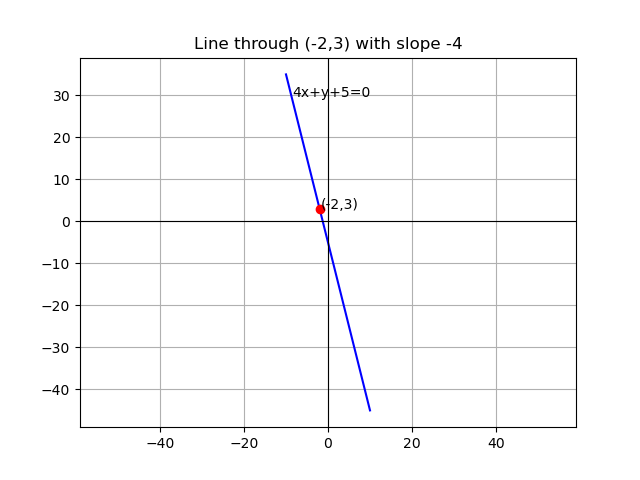
\includegraphics[width=0.9\columnwidth]{figs/fig6.png}
\caption{fig : Representation of Line and Point}
\label{Fig6}
\end{figure}
\end{frame}
\section{C Code}
\begin{frame}[fragile]
\frametitle{C Code }
\begin{lstlisting}[language=C]
#include <stdio.h>
// Function to print line equation given point (x0,y0) and slope
void line_equation(double x0, double y0, double slope) {
    // direction vector from slope
    double dx = 1.0;
    double dy = slope;
    // normal vector = (dy, -dx)
    double a = dy;
    double b = -dx;
    double c = -(a * x0 + b * y0);

    printf("Point on line: (%.2f, %.2f)\n", x0, y0);
    printf("Slope: %.2f\n", slope);
    printf("Cartesian form: %.2fx + %.2fy + %.2f = 0\n", a, b, c);
    printf("Vector form: r = (%.2f, %.2f) + t(%.2f, %.2f)\n",
           x0, y0, dx, dy);
}
\end{lstlisting}
\end{frame}
\begin{frame}[fragile]
\begin{lstlisting}
// Function exposed for Python (shared object)
const char* get_line_equation() {
    static char result[200];
    double x0 = -2, y0 = 3, slope = -4;
    double dx = 1.0, dy = slope;
    double a = dy, b = -dx, c = -(a * x0 + b * y0);

    snprintf(result, sizeof(result),
             "Equation: %.2fx + %.2fy + %.2f = 0; Vector: r = (%.2f, %.2f) + t(%.2f, %.2f)",
             a, b, c, x0, y0, dx, dy);
    return result;}
int main() {
    // Example: line through (-2,3) with slope -4
    line_equation(-2, 3, -4);
    return 0;
}  
\end{lstlisting}
\end{frame}

\section{Python Code}
\begin{frame}[fragile]
\frametitle{Python : call\_c.py}
\begin{lstlisting}
import ctypes
import os

# Part 1: Call the C shared object
# Path to shared object (must be in same directory)
lib_path = os.path.abspath("./libline.so")

# Load the shared library
lib = ctypes.CDLL(lib_path)

# Tell Python return type of the function
lib.get_line_equation.restype = ctypes.c_char_p
# Call the function
c_result = lib.get_line_equation().decode("utf-8")
print("=== Result from C shared library ===")
print(c_result)
\end{lstlisting}
\end{frame}
\begin{frame}[fragile]
\begin{lstlisting}
print()
# Part 2: Direct computation in Python

def line_equation(x0, y0, slope):
    dx, dy = 1.0, slope
    a, b = dy, -dx
    c = -(a * x0 + b * y0)
    print("=== Direct Python Computation ===")
    print(f"Point on line: ({x0}, {y0})")
    print(f"Slope: {slope}")
    print(f"Cartesian form: {a:.2f}x + {b:.2f}y + {c:.2f} = 0")
    print(f"Vector form: r = ({x0}, {y0}) + t({dx}, {dy})")
    print()

line_equation(-2, 3, -4)

# Part 3: Row reduction (manual)
def row_reduction():
\end{lstlisting}
\end{frame}
\begin{frame}[fragile]
\begin{lstlisting}
    print("=== Row Reduction Verification ===")
    # Equations: a - 4b = 0, -2a + 3b + c = 0
    print("System of equations:")
    print("1) a - 4b = 0")
    print("2) -2a + 3b + c = 0")

    # From (1): a = 4b
    # Substitute into (2): -8b + 3b + c = 0 => -5b + c = 0 => c = 5b
    a = 4
    b = 1
    c = 5
    print(f"Solution (up to scale): (a, b, c) = ({a}, {b}, {c})")
    print(f"Equation: {a}x + {b}y + {c} = 0")
    print()

row_reduction()

\end{lstlisting}
\end{frame}

\begin{frame}[fragile]
\frametitle{Python Code for Plotting}
\begin{lstlisting}[language=Python]
import numpy as np
import matplotlib.pyplot as plt
x=np.linspace(-10, 10, 100)
y=(-4*x)-5

plt.plot(x, y, '-b')
plt.plot(-2, 3, 'ro')
plt.text(-8.6, 29.6, "4x+y+5=0", fontsize=10, color="black")
plt.text(-1.8, 2.9, "(-2,3)", fontsize=10, color="black")
plt.axhline(0, color="black", linewidth=0.8)
plt.axvline(0, color="black", linewidth=0.8)
plt.title("Line through (-2,3) with slope -4")
plt.grid(True)
plt.axis("equal")
plt.savefig("../figs/fig6.png")
plt.show()
\end{lstlisting}
\end{frame}

\end{document}
  
